We first introduce the data sets on which we conduct our experiments, and describe the experimental setup. We then describe our methodology for comparing the performance of various algorithms for the affiliation recommendation task. 
Finally, we present a series of experiments using methods presented in previous sections, and discuss the results. 

\subsection{Data}
We use two popular online social networks  for our experiments. These are \textit{Orkut} and \textit{Youtube}, and both are operated by Google. The users of both social networks explicitly identify themselves as belonging to some \textit{communities} or \textit{groups}. Thus, for each of the networks we have adjacency matrix $\A$ that identifies the memberships of the users in the groups and adjacency matrix $\SS$ that identifies friendships among users. For our experiments, we used data gathered by \cite{Mislove}. We compare the predictive ability of the algorithms using these large networks. In a few of the experiments we used the largest connected component, denoted with Okrut-1c and Youtube-1c, as path based measures, e.g. \textsf{Katz}, are decoupled and indepedent for different components. Some statistics for these networks are presented in Table \ref{tab:datasets}.

\begin{table}[ht!]
\centering
\begin{tabular}{| l | r | r | r | r |} \hline
Feature & Orkut & Youtube & Orkut-1c & Youtube-1c\\ \hline
Number of users, $N_{u}$ & 9123 & 16575 & 9123 & 16535\\ \hline
Number of groups, $N_{g}$ & 75546 & 21326 & 20905 & 17672\\ \hline
Average number of groups per user & 55.8 & 10.5 & 25 & 10.2\\ \hline
Minimum number of groups per user & 4 & 4 & 0 & 2\\ \hline
% Mode of number of groups per user & 6 & 4 & 6 & 4\\ \hline
Average number of users per group & 6.7 & 8.1 & 10.9 & 9.6\\ \hline
% Mode of number of users per group & 2 & 1 & 1 & 1\\ \hline
Minimum number of users per group & 1 & 1 & 2 & 1\\ \hline
Average number of friends per user & 46 & 11.7 & 46 & 11.7\\ \hline
% Mode of number of friends per user & 2 & 1 & 2 & 1\\ \hline
\end{tabular}
\caption{Some statistical properties of the data sets used in our experiments. The Orkut-1c and Youtube-1c are the largest connected components from the Orkut and Youtube networks, respectively.}
\label{tab:datasets}
\end{table}

\subsection{Experiment setup}
For every user $u$ and a group $g$, let $\E_u = \set{(u,g) \ | \ \A_{u,g} = 1}$ denote the affiliations of $u$, as observed in a given affiliation network $\A$. Invariably, in all the experiments, we set aside a subset of these affiliations $\E_{u}^{(t)} \subset \E_u$ as test data. We use $|\E_u^{(t)}| = 30 \% |\E_u|$. The remaining affiliations $\E_u^{(tr)} = \E_u \setminus \E_u^{(t)}$ are used as training data for the recommendation algorithms.

All of our recommendation algorithms require ``learning'' parameters for some model of the affiliation process, and hence for the purposes of learning the parameters, we use a set of \textit{validation} links $\E_u^{(v)} \subset \E_u^{(tr)}$ with $|\E_u^{(v)}| = 30 \% |\E_u^{(tr)}|$. During the validation process, we compare different model parameters based on the number of correct edges among $25 N_u$ recommendations\footnote{$25 N_u$  is chosen because, in Section \ref{Evaluation method}, we argue that a predictive model should be judged based on the quality of its top few recommendations.} made using a model.

\subsubsection{Evaluation method}
\label{Evaluation method}
We now describe our methodology for evaluating the performance of an affiliation recommendation algorithm. We first introduce notions of interest, such as \textit{precision}, \textit{recall}, \textit{sensitivity}, \textit{specificity}, \textit{ROC} (receiver operating characteristic) and \textit{AUC} (area under curve). We then describe the way in which we evaluate the performance of a recommendation algorithm based on its top 50 recommendations to the average user. We then demonstrate the importance of choosing the right evaluation method for the community recommendation task by showing that using a different, but less appropriate, evaluation strategy yields different results.

\subsubsection{Performance Measures}
Three commonly used measures of quality of solutions in information retrieval and classification tasks are \textit{precision}, \textit{recall} or \textit{sensitivity} and \textit{specificity}. Precision measures the exactness or fidelity of the prediction while sensitivity measures the completeness of the prediction. Suppose that the recommendation algorithm makes $n$ recommendations to a user. Then, precision is defined as the ratio of the number of correctly identified positives (true positives) to $n$, and sensitivity is the ratio of the number of correctly identified positives to the total number of positives, i.e. $|\E_u^{(t)}|$. Specificity, on the other hand, measures the ability of the recommender to exclude uninteresting affiliations from the recommendations it makes. It is defined as the fraction of such ``negative affiliations'' correctly excluded from the recommendation. All three of these performance measures range from zero to one.

\subsubsection{ROC---Receiver Operating Characteristic}
Often, one is interested in evaluating the performance of a recommendation algorithm not for a single value of the number of recommendations~$n$, but for the entire range of $n$. For a given recommendation algorithm and a user, sensitivity is a non-decreasing function of $n$. The relationship between the increase in sensitivity, as $n$ increases, with the decrease in specificity is of interest in comparing the quality of recommendations. For a good recommendation, as $n$ increases, sensitivity increases without a big drop in specificity. The ROC curve is a plot of the sensitivity vs $(1 - \text{specificity})$ for all values of~$n$. It is a common way of comparing the performance of classification algorithms over the entire range of $n$ (or equivalently cutoff scores). The AUC curve (area under the ROC curve), is then used as a way to compare different classification algorithms: the greater the AUC, the better the algorithm's sensitivity vs $(1-\text{specificity})$ tradeoff.

Consider a social network website, like Orkut or Facebook; or a vendor like Netflix which sells movies. They would be interested in making, let us say, five pages of recommendations to their users, but not much more than that. Certainly not a hundred. Also, irrespective of whether a user participates in five communities or seventy, the social networking website would probably want to make roughly the same number of recommendations per user. So, we choose to evaluate the recommendation algorithms we propose based on their top 50 recommendations. 
We do this by examining the portion of the ROC curve obtained by measuring the sensitivity and specificity the recommendation algorithm achieves for an average user at regular intervals between $n = 1$ and $n = 50$. To do this, for a given $n$ between 1 and 50, we compute the sensitivity and specificity for every user in the network, and take the mean of these values to be the average sensitivity and average specificity for that $n$.\footnote{So, both average sensitivity and average specificity may be viewed as functions of the number of recommendations $n$.} We then plot the average sensitivity vs $(1 - \text{average specificity})$ curve, as in Figure \ref{fig:summaryResults}. Note that comparisons made using this method are statistically robust, as the sensitivities and specificities of recommendation algorithms are averaged over, e.g., 9500 users in Orkut and 16000 users in Youtube.

\subsubsection{``Global'' vs ``per-user'' sensitivity}
\label{sec:globalVsPerUserEvaluationMethods}
Let $k(n_u)$ be the number of ``good recommendations'' made by a recommendation algorithm for a user $u$, when it makes $n_u$ recommendations to that user. Then, ``per user'' sensitivity measure is defined as 
%$N_u^{-1} \sum_u \displaystyle\frac{k(n_u) }{|\E_u^{(t)}|}$. 
$N_u^{-1} \sum_u  ( k(n_u) / |\E_u^{(t)}|)$. 
In our experiments, we will use $n_u = 50\; \forall u$. Contrast this with finding the ``global'' sensitivity 
%$\dfrac{k'(n)}{\sum_u |\E_u^{(t)}|}$, 
$k'(n) / ( \sum_u |\E_u^{(t)}|)$, 
where $k'(n)$ denotes the number of ``good recommendations'' made by a given recommendation algorithm while making $n$ predictions in total. For a fixed $n$, this ``global'' sensitivity is proportional to precision, and is a commonly used measure of performance of link prediction algorithms in the context of social network analysis. Note that, in this case, while $n = \sum_u n_u$, there is no guarantee that, for two given users $u$ and $v$, $n_u = n_v$; indeed the recommendation algorithm, when asked to make $n$ recommendations, may not make any recommendations at all for some users. Therefore, this measure of goodness of a recommendation algorithm is not equivalent to the ``per user'' sensitivity.

Judging identical algorithms on identical data sets, using these alternative evaluation methods can yield very different rankings of recommendation algorithms, as illustrated by comparing Figure~\ref{fig:linkPredictionEvaluation} with Figure~\ref{fig:summaryResults}. Hence, the choice of an appropriate method for evaluating affiliation recommendations is an important one.

\begin{figure}[h]
  \begin{center}
    \subfigure[Orkut data set]{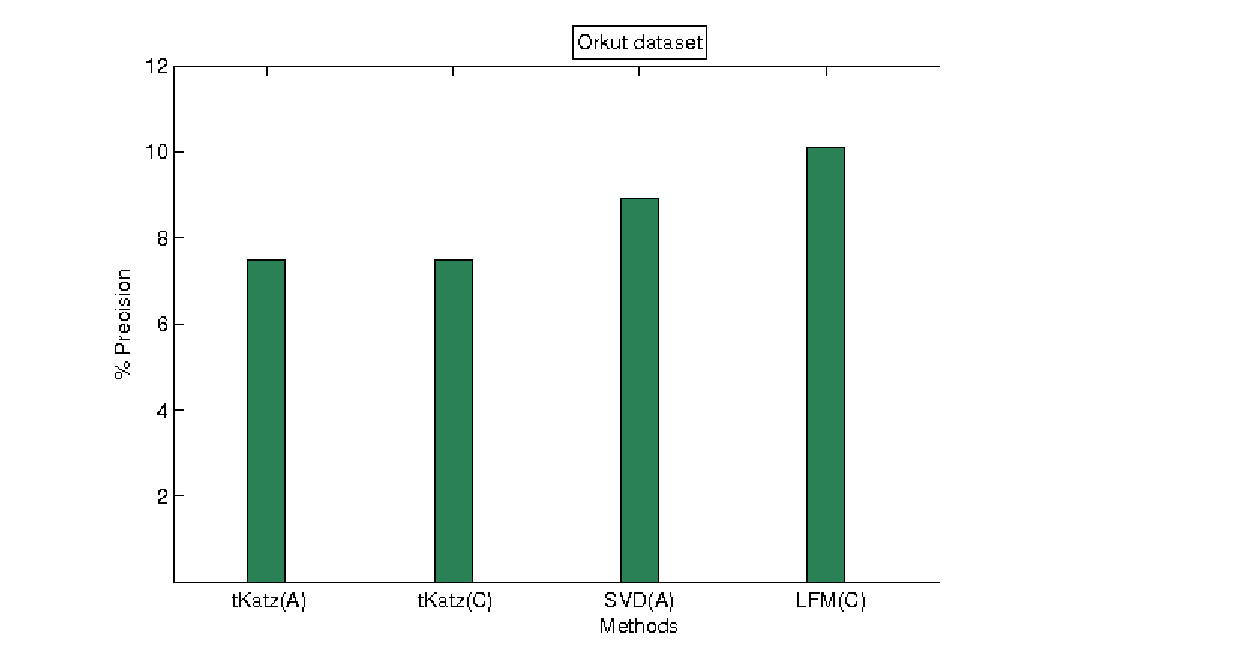
\includegraphics[scale=0.35]{OrkutLinkPredictionEvaluation.eps}}
    \subfigure[Youtube data set]{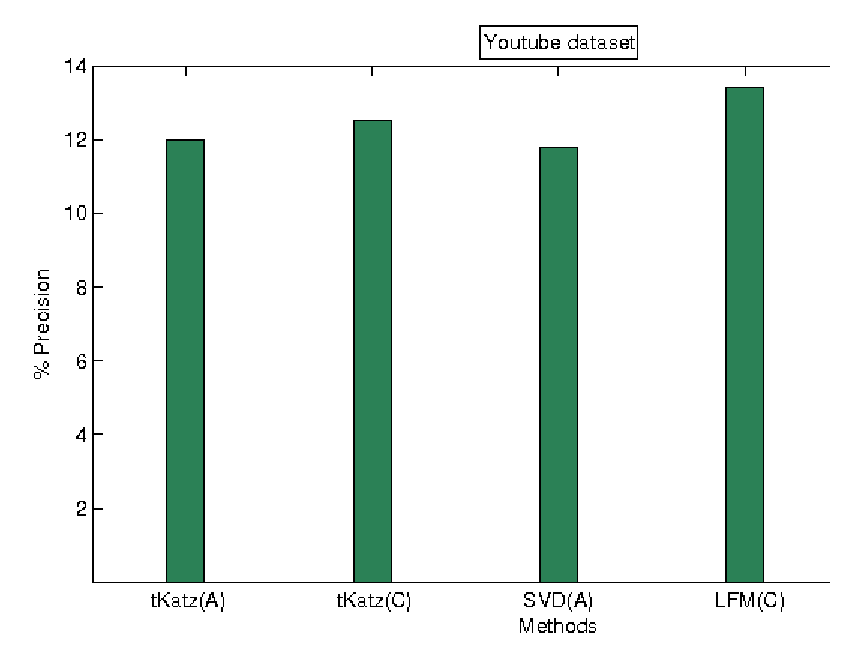
\includegraphics[scale=0.35]{YoutubeLinkPredictionEvaluation.eps}}
  \end{center}
  \caption{In this figure, various recommendation algorithms are compared using the ``global'' sensitivity measure described in Section \ref{sec:globalVsPerUserEvaluationMethods}, where a total of $\sum_u E_u$ recommendations are made, with no guarantees about the number of recommendations made for any given user. According to this evaluation method, LFM($\C$) appears to be superior to \textsf{tKatz}($\C$). However, these results are different from those described in Figure \ref{fig:summaryResults}, where recommendation algorithms are compared based on the goodness of the top 50 recommendations made for the average user.}
  \label{fig:linkPredictionEvaluation}
\end{figure}

\begin{figure}[ht]
  \begin{center}
    \subfigure[Orkut data set]{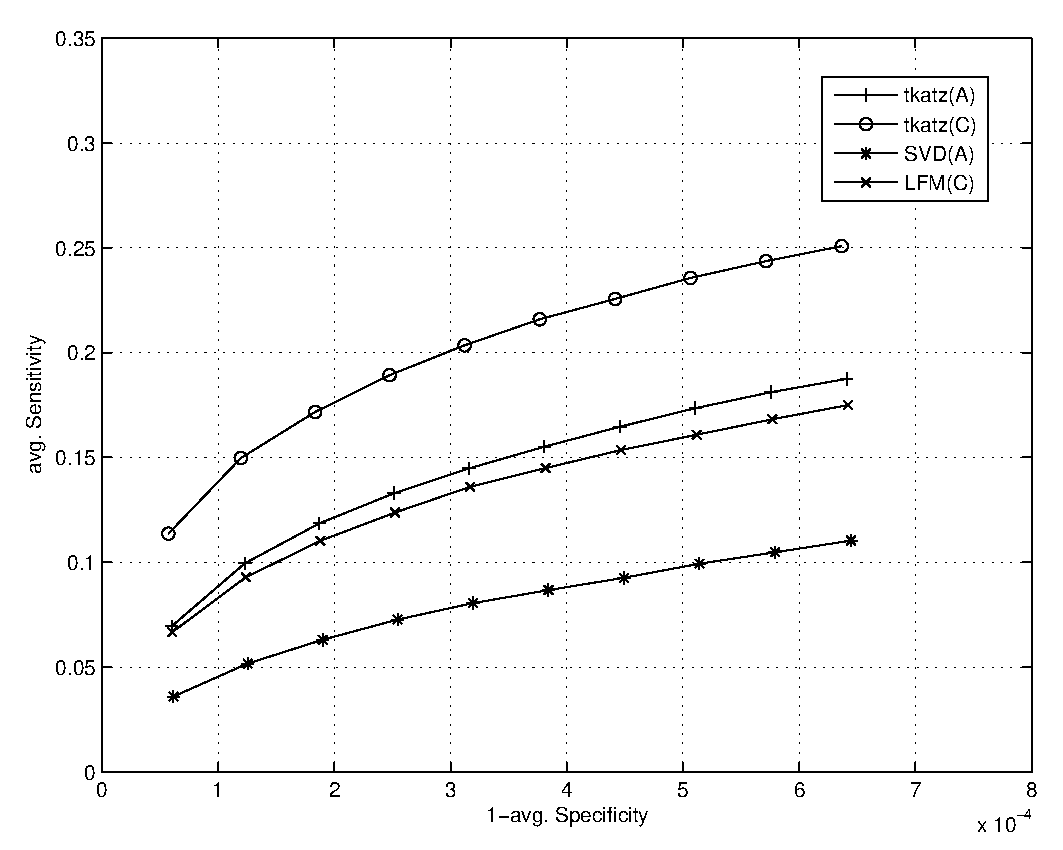
\includegraphics[scale=0.35]{summaryOrkut.eps} \label{fig:sumRes-a}}
    \subfigure[Youtube data set]{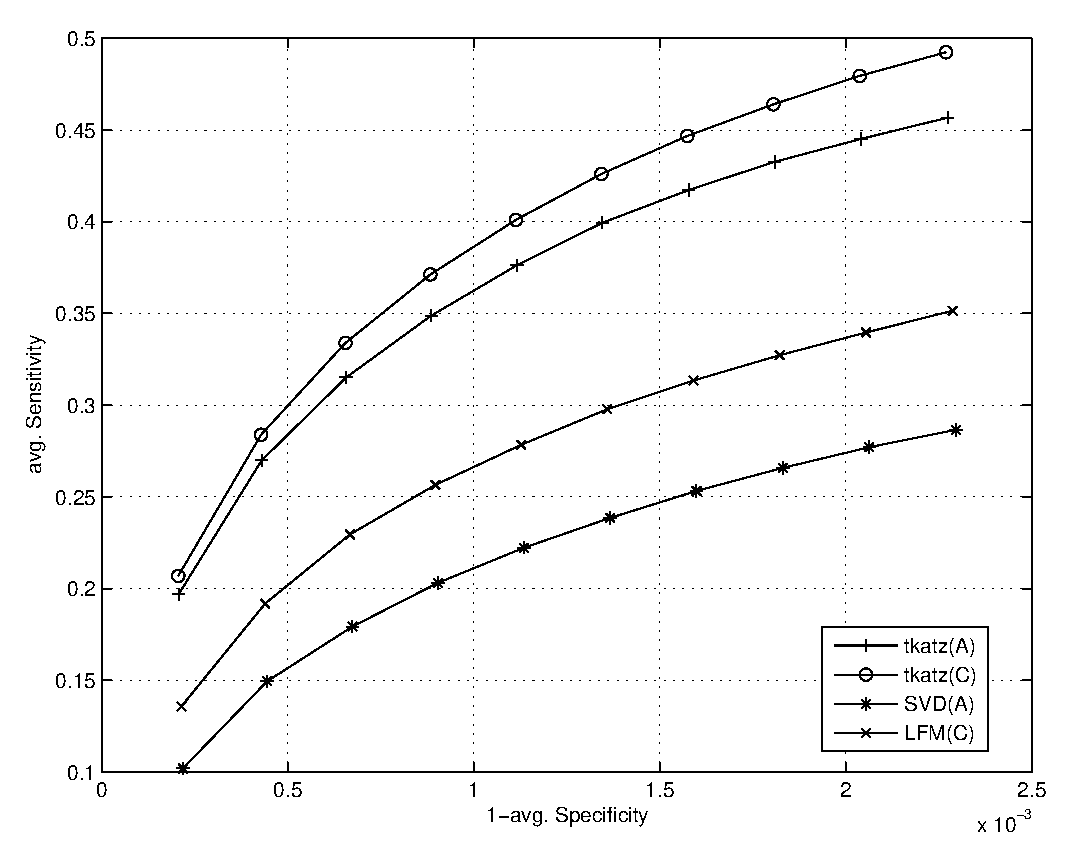
\includegraphics[scale=0.35]{summaryYoutube.eps}\label{fig:sumRes-b}}
  \end{center}
  \caption{Comparison of recommendation algorithms based on graph proximity and latent factors models, as described in Section \ref{Evaluation method}. The leading portion of the ROC curve is shown, thus recommendation algorithms are compared based on the goodness of their top 50 recommendations. The graph proximity based predictors consistently outperform latent factors based predictors in the two data sets. See Section \ref{Results and Discussion} for further discussion.}
  \label{fig:summaryResults}
\end{figure}

\begin{figure}[ht]
  \begin{center}
    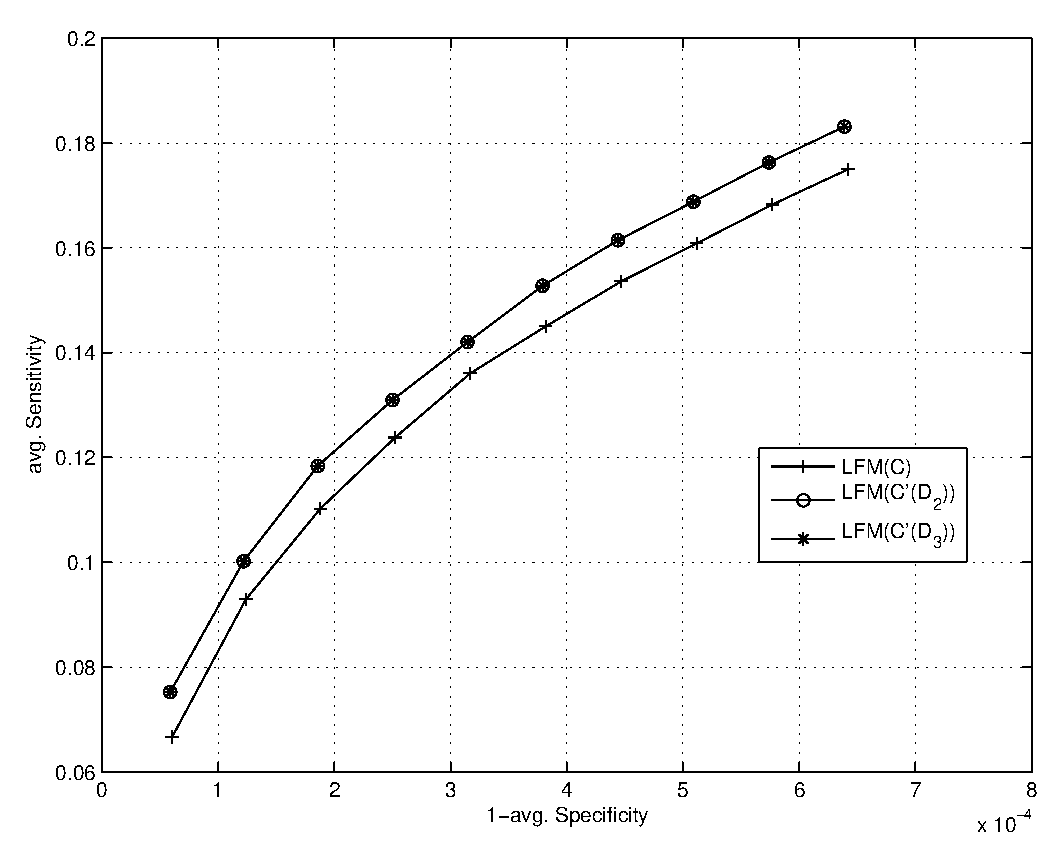
\includegraphics[scale=0.66]{summarySVDOrkut.eps}
  \end{center}
  \caption{Comparison of latent factors based algorithms for various choices of $\D$, for the Orkut data set: $\D_{2} = \A^{T}\A, \D_{3} = \lambda \A^{T}\A$.}
  \label{fig:summarySVD}
\end{figure}


\subsection{Results and Discussion}
\label{Results and Discussion}
\begin{table}[h!]
\centering
\begin{tabular}{| c | l |} \hline
\textsc{Experiment}&\textsc{Score Matrix}\\ \hline
\textsf{tKatz}(\A) & \textsf{tKatz}$(\A\A^T, \beta, k) \A$ \\ \hline
\textsf{tKatz}(\C) & Equation (\ref{e:tKatzC}) \\ \hline
SVD(\A) & SVD(\A) \\ \hline
LFM(\C) & Equation (\ref{e:LFM}) \\ \hline
LFM-c(\C, $c$) & Equation (\ref{e:clustLowRankC}) extended to $c$ clusters\\ \hline
\textsf{tKatzCS}($d$) & Equation (\ref{e:tKatzCS}) \\ \hline
\textsf{tKatzLFM}(\C, $d$) & \textsf{tKatz}($\C_d$), where $\C_d$ is rank-$d$ approximation of \C \\ \hline
\textsf{tKatzLFM-c}(\C, $c$, $d$)) & \textsf{tKatz}($\C_d$), where $\C_d$ is the clustered rank-$d$ approximation of \C \\ \hline
\end{tabular}
\caption{List of experiments, with the score matrix used for ranking the user-group connections, based on latent factor and graph proximity models.}
\label{tab:experiments}
\end{table}

In this section, we report and analyse the performance of the various recommendation algorithms, based on the graph proximity model and latent factors model discussed in Sections \ref{Models} and \ref{Scalability}. We compare the performance of the graph proximity methods with the latent factors methods on the average sensitivity and average specificity metrics introduced earlier, for a given number of recommendations in $\{ 5,10,\cdots,45, 50\}$.  We study the performance of the scalable approximation methods proposed in Section \ref{Scalability}, and compare these methods amongst themselves and with the methods proposed in Section \ref{Models}. The list of experiments based on latent factor and graph proximity predictors are presented in Table \ref{tab:experiments}.

\subsubsection{Performance of recommenders based on the two models}
Consider the performance of the recommendation algorithms on the Orkut data set in Figure \ref{fig:sumRes-a}. SVD($\A$) gives the lowest performance of all the methods. LFM($\C$) performs better than SVD($\A$), which is expected given that it uses information from the friendship network $\SS$ in addition to the information from affiliation network $\A$. For the average user, the graph proximity model based methods significantly outperform latent factors based methods as observed in both plots of Figure \ref{fig:summaryResults}. In particular, we see that \textsf{tKatz}($\C$) performs much better than \textsf{tKatz}($\A$), which in turn outperforms latent factor based methods. We see that the information in the friendship network indeed proves highly beneficial in making affiliation recommendations and graph proximity based methods exploit this information the most. A summary of performances of the algorithms on the Youtube data set are shown in Figure \ref{fig:summaryResults} (b). We observe that the case for Youtube is similar to that of Orkut, in that graph proximity based algorithms significantly outperform latent factors based algorithms. In particular, \textsf{tKatz}($\C$) is highly successful compared to the other methods. 


Another interesting comparison of latent factor methods based on the choice of $\D$ in constructing the combined network $\C'$ given in (\ref{e:generalizedCombined}), is presented in Figure \ref{fig:summarySVD}. We observe that the choice of $\D$ does not appear to make any significant difference in the performance of the recommendation algorithm. In the plot we use $\D_2 = \A^{T}\A$ and $\D_3 = \lambda \A^{T}\A$, where $\lambda$ is also the weight associated with $\SS$ in the combined graph. Even though, in case of the Orkut data set, we see that SVD($\C', \D$) performs slightly better than SVD($\C$), it appears as if scaling $\D \neq 0$ does not affect recommendation quality. In case of Youtube (plots not shown), our experiments indicate that $\D$ is not useful at all. The obvious choices for $\D$ do not seam to improve the performance compared with $\D = 0$.


The best parameters learned by the various algorithms are presented in Table~\ref{tab:parameters}. Note that the best parameter $\beta = 10^{-12}$ implies that the calculated \textsf{tKatz} measure was effectively using the common neighbors method. In other words, users and communities connected by path lengths 5 or more\footnote{Corresponding to 2nd and higher powers of $\beta \A\A^{T}$ in \textsf{tKatz}(\A).} are not useful in making affiliation recommendations.

\begin{table}[t!]
\centering
\begin{tabular}{| c | p{2.4cm} | p{2.4cm} |} \hline
Algorithm&Orkut&Youtube\\ \hline
LFM($\C$) & $d=50, \gl = 0.8$ & $d = 90, \gl = 1$ \\ \hline
LFM($\C'(\lambda \A^{T} \A)$) & $d = 60, \gl = 0.6$ & $d = 70, \gl = 1$ \\ \hline
\textsf{tKatz}($\A$) & $\gb = 10^{-12}$ & $\gb = 10^{-12}$ \\ \hline
\textsf{tKatz}($\C$) & $\gb = 0.01, \gl = 0.2$ & $\gb = 0.1, \gl = 0.4$ \\ \hline
\end{tabular}
\caption{Best parameters learned by the recommendation algorithms using validation.}
\label{tab:parameters}
\end{table}

We see that the recommendation algorithms perform consistently across the two data sets, and the evaluations are robust as the specificities and sensitivities are averaged over 9000 users in Orkut and 16000 users in Youtube.

\subsubsection{Scalable approximations to \textsf{tKatz}(C)}
From Figure \ref{fig:summarySVDKatz}, we observe that in general, combining ideas from the latent factor model with graph proximity model yields better performance than simply using the low rank approximations of $\C$. The exception to this is the case of recommendations made by LMF-c on the Orkut-1c data set, here \textsf{tKatzLMF-c} decreases the quality of the predictions made by LMF-c further.

In Figure \ref{fig:summaryScalability}, we observe that the recommendation quality of the scalable recommenders proposed in this paper is close to that of \textsf{tKatz}($\C$). In particular, we note that \textsf{tKatzCS} consistently performs very well on both data sets. Comparing the performance of \textsf{tKatzLFM} and \textsf{tKatzLFM-c}, we also note that the use of clustering is effective in improving performance, and this suggests that we can perhaps derive similar benefit out of considering a clustered version of the \textsf{tKatzCS} algorithm.

Finally, in Figure \ref{fig:summaryDependency}, we study the effects of change in the number of clusters and the number of factors used on the performance of algorithms which use graph clustering for the purpose of scalability. We observe that changing the number of clusters does not make a significant difference in performance, whereas increasing the number of factors yields better performance. This is not surprising considering the fact that these algorithms can be viewed as computing approximations of \textsf{tKatz}($\C$).

\begin{figure}[ht]
  \begin{center}
    \subfigure[Orkut-1c data set]{\includegraphics[scale=0.35]{summarySVDKatzOrkut.eps}}
    \subfigure[Youtube-1c data set]{\includegraphics[scale=0.35]{summarySVDKatzYoutube.eps}}
  \end{center}
  \caption{In this figure, we observe that, in general, combining ideas from the latent factor model with ideas from the graph proximity model yields better performance than simply using the low rank approximations of $\C$ in isolation. This is consistent with our observations in Figure \ref{fig:summaryResults}. See Section \ref{Results and Discussion} for further discussion.}
  \label{fig:summarySVDKatz}
\end{figure}

\begin{figure}[ht]
  \begin{center}
    \subfigure[Orkut-1c data set]{\includegraphics[scale=0.35]{summaryScalabilityOrkut.eps}}
    \subfigure[Youtube-1c data set]{\includegraphics[scale=0.35]{summaryScalabilityYoutube.eps}}
  \end{center}
  \caption{Comparison of the performance of the proposed scalable graph proximity based methods. In this figure, we observe that the recommendation-quality of the scalable recommenders proposed in this paper is close to that of \textsf{tKatz}($\C$). In particular, we note that \textsf{tKatzCS} consistently performs very well on both data sets. Comparing the performance of \textsf{tKatzLFM} and \textsf{tKatzLFM-c}, we also note that the use of clustering is effective in improving performance.}
  \label{fig:summaryScalability}
\end{figure}


\begin{figure}[ht]
  \begin{center}
    \subfigure[Effect of changing the number of clusters.]{\includegraphics[scale=0.35]{summaryClusteredMethodsClusterDependencyYoutube.eps}}
    \subfigure[Effect of changing the number of factors.]{\includegraphics[scale=0.35]{summaryRankDependencyYoutube.eps}}
  \end{center}
  \caption{In this figure, we study the effects of change in the number of clusters and the number of factors used on the performance of algorithms which use graph clustering for the purpose of scalability. These experiments were conducted on the Youtube-1c data set. We observe that changing the number of clusters does not make a significant difference in performance, whereas increasing the number of factors yields better performance. This is not surprising considering the fact that these algorithms can be viewed as computing approximations of \textsf{tKatz}($\C$).}
  \label{fig:summaryDependency}
\end{figure}


%\begin{table}[ht]
%\centering
%\begin{tabular}{| c | p{2.4cm} | p{2.4cm} |} \hline
%Algorithm& Runtime\\ \hline
%SVD($\C$)& 71.4\\ \hline
%SVDcl($\C$, 5) & 191.1\\ \hline
%tKatz($\A$)& 27.3\\ \hline
%tKatz($\C$)& 96.2\\ \hline
%tKatz(SVD($\C$))& 90.3\\ \hline
%tKatz(SVD($\A$, 300), SVD($\SS$, 300))& 1160\\ \hline
%tKatz(SVDCl($\C$, 300))& 644\\ \hline
%\end{tabular}
%\caption{Run-times in seconds of various algorithms on a 2.5GHz machine with 512KB cache.}
%\label{tab:runTimes}
%\end{table}


